% figure: 777-7-11-ans-采样节点与信号.png
% Original topology: question booklet p.126 (PDF p.132).
% The two ideal samplers share period T and sampling instants.
\documentclass[border=9pt]{standalone}
\usepackage{fontspec}
\setmainfont{Cambria}
\usepackage{unicode-math}
\setmathfont{Cambria Math}
\usepackage{tikz}
\usetikzlibrary{arrows.meta}
\begin{document}
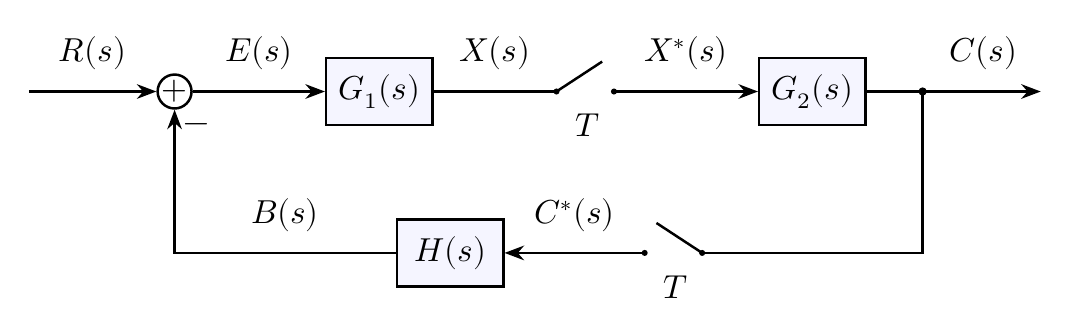
\begin{tikzpicture}[>=Stealth,line width=0.9pt,
  block/.style={draw,minimum width=1.35cm,minimum height=0.85cm,fill=blue!4},
  sum/.style={draw,circle,minimum size=0.43cm,inner sep=0pt},
  every node/.style={font=\large}]
\node[sum] (sum) at (0,0) {$+$};
\node[block] (g1) at (2.6,0) {$G_1(s)$};
\node[block] (g2) at (8.1,0) {$G_2(s)$};
\node[block] (h) at (3.5,-2.05) {$H(s)$};
\draw[->] (-1.85,0) -- node[above=4pt] {$R(s)$} (sum.west);
\draw[->] (sum.east) -- node[above=4pt] {$E(s)$} (g1.west);
\draw (g1.east) -- node[above=4pt] {$X(s)$} (4.85,0);
\fill (4.85,0) circle (1.1pt);
\draw (4.85,0) -- (5.43,0.38);
\fill (5.58,0) circle (1.1pt);
\draw[->] (5.58,0) -- node[above=4pt] {$X^{\ast}(s)$} (g2.west);
\node at (5.22,-0.43) {$T$};
\draw[->] (g2.east) -- node[above=4pt,pos=0.67] {$C(s)$} (11,0);
\fill (9.5,0) circle (1.5pt);
\draw (9.5,0) -- (9.5,-2.05) -- (6.7,-2.05);
\fill (6.7,-2.05) circle (1.1pt);
\draw (6.7,-2.05) -- (6.12,-1.67);
\fill (5.97,-2.05) circle (1.1pt);
\draw[->] (5.97,-2.05) -- node[above=4pt] {$C^{\ast}(s)$} (h.east);
\node at (6.33,-2.48) {$T$};
\draw[->] (h.west) -- node[above=4pt] {$B(s)$} (0,-2.05) -- (sum.south);
\node at (0.28,-0.46) {$-$};
\end{tikzpicture}
\end{document}
